\section{Answers to Assignment Questions}

\noindent \textbf{Q1. After DROPping echo-reply packets on OUTPUT chain, what 
was the observed effect? Use Figure~\ref{fig:icmpexampleQ1} to illustrate the 
path of the packets. Mark the path with arrows and use an X to mark the point 
where the packets are DROPped.}
~\ \\

The host is receiving incoming echo requests and replies with and echo reply. However, outgoing echo replies are dropped when matching the newly created rule (as marked by the red X in figure \ref{fig:icmpexampleQ1} ).
~\ \\

\noindent \textbf{Q2. After DROPing echo-request packets on INPUT chain, what
was the observed effect? How is this reaction different from the reaction
achieved in Q1? Use Figure~\ref{fig:icmpexample} to illustrate the path of 
the
packets. Mark the path with arrows and use an X to mark the point where the
packets are DROPped.}
~\ \\

This time around incoming echo requests will be blocked going in to our host.
~\ \\

\begin{figure}[!ht]
    \begin{center}
        \subfigure[Use this Figure to explain Q1]{
            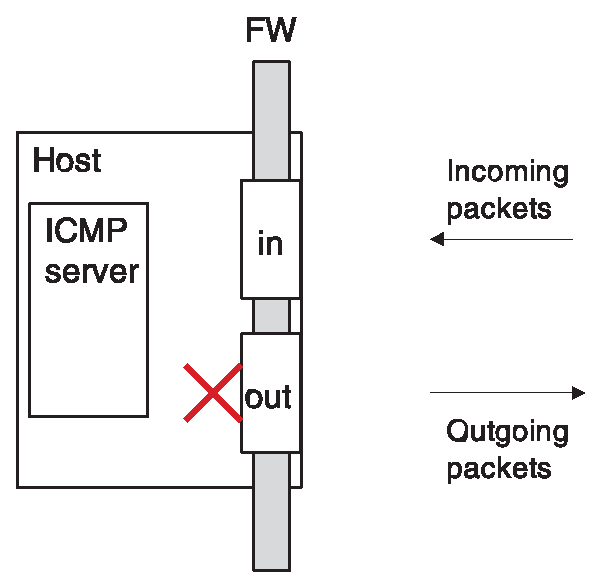
\includegraphics[scale=0.5]{figures/icmpexampleQ1.eps}
            \label{fig:icmpexampleQ1}
        }
        \hspace{1in}
        \subfigure[Use this Figure to explain Q2]{
            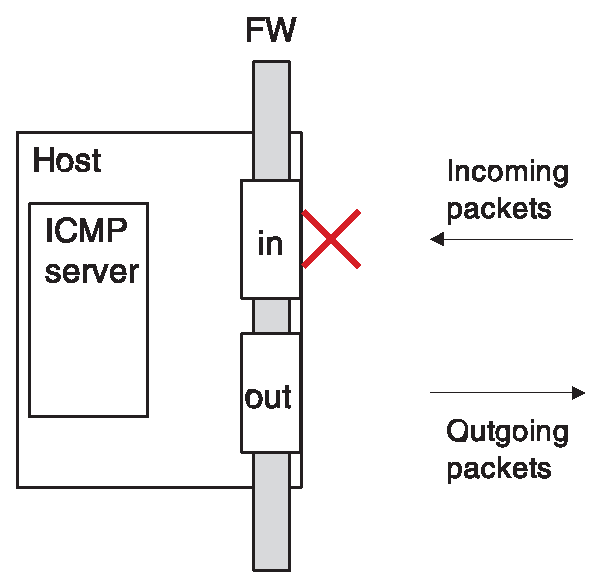
\includegraphics[scale=0.5]{figures/icmpexampleQ2.eps}
            \label{fig:icmpexampleQ2}
        }
    \end{center}
    \caption{Figure to help you illustrate your thoughts regarding the packet 
        flow in questions Q1 and Q2.}
    \label{fig:icmpexample}
\end{figure}

\noindent \textbf{Q3. For each entry in the log, several information items are
displayed. Some entries can be useful for creating new rules. Explain the 
items \texttt{IN}, \texttt{OUT}, \texttt{SRC}, \texttt{DST} and \texttt{PROTO}
mean and why these might be useful.}
~\ \\

IN and OUT denotes on what physical interface the packet entered and/or exited. SRC and DST represents the source and destination ip addresses respectively. PROTO is the protocol used on the network layer. This can be either TCP or UDP. (Table??)
~\ \\

\noindent \textbf{Q4. At this stage, with default policy set to DROP for all 
chains, would you consider the system secure? Would you consider it useful?}
~\ \\

The system is indeed more secure with the default policy set to DROP, not allowing any traffic going either in or out. In the aspect of being useful, a local user would not be permitted to browse the web or even check their mail at this stage.
~\ \\

\noindent \textbf{Q5. Assume instead that you used default policy ACCEPT, 
would you consider the system secure now? Would you consider it useful?}
~\ \\

With a default policy set to ACCEPT the system would be less secure. Having no control over who has access or from where. Local users and processes would not have any issue connecting to the outside world making it convenient. 
~\ \\

\noindent \textbf{Q6. You just added some protection against flooding by 
limiting the number of packets the firewall will let through to 1 per second. 
Give two examples on how you can tell that you are protected!}
~\ \\

Using the ping command we can try to send, for example, five ICMP echo-request packets per second. If the sequence number on the echo-reply packets are inconsistent we then know that some packets were dropped by the firewall.
We can also check the current configuration to see how many packets matched the new rule with \texttt{sudo iptables -vL}. The output should list a number of packets
~\ \\
